\documentclass[8pt]{beamer}
\setbeamertemplate{caption}{\raggedright\insertcaption\par} % Without prefix "Figure"
\usepackage{graphics}
\title{Auto-correlations of spins in 1D East Model}
\author{Gang Huang}
\usetheme{Frankfurt}
\definecolor{mygreen}{rgb}{.3,.4,.12}
\usecolortheme[named=mygreen]{structure}

% Add page number
\setbeamertemplate{sidebar right}{}
\setbeamertemplate{footline}{%
	\hfill\usebeamertemplate***{navigation symbols}
	\hspace{1cm}\insertframenumber{}/\inserttotalframenumber}

\begin{document}
\maketitle

\section{1D East Model}
\begin{frame}
	\frametitle{East Model is an example of kinetically constrained Ising model.} 
	East model is a 1-D system of spins on lattice. For site $i$, $n_i =0$ or 1. 	No static interactions between spins. (\textbf{Palmer 1984; Jaeckle, Eisinger 1991; Eisinger, Jaeckle 1993; Faggionato, Martinelli, Roberto, and Toninelli 2012 })
	
	Boundary condition:  PBC (\textbf{Sollich,2003}). 
	

	
	A given spin may only flip if the neighboring spin to the right is up, with an acceptance ratio $A$,
     \begin{alignat}{3}
       A = \left\{
       \begin{aligned}
	     e^{-\beta}, \text{ for } 01 \to 11 \\
         1, \text{ for } 11 \to 01.
       \end{aligned}
       \right
       .
     \end{alignat}
 East model shows glassy dynamics. (\textbf{Pitts and Andersen, 2001})
 %ie., its relaxation properties are similar to those of glass forming liquids and because some of them undergo ergodic–nonergodic transitions. 
 
 Auto-correlation function
      \begin{alignat}{3}
      C(t) = \frac{\langle\delta n_i(t)\delta n_i (0)\rangle}{\langle \delta n_i(0)^2 \rangle} = \frac{\langle n_i(t)n_i(0)\rangle - c^2}{c-c^2} = \frac{\langle\delta n_i(t)\delta n_i (0)\rangle}{c(1-c)}  .
 \end{alignat}
$\langle \cdots \rangle$: Average for the equilibrium state; $n_i$: occupation number of site $i$; $c = \langle n_i \rangle$; $\langle n_i(t)^2 \rangle = \langle n_i(t)\rangle$.
\end{frame}

\begin{frame}
	\frametitle{Relation between $\beta$ and $c$}
	Denote $c = \langle n_i \rangle_{\text{eq}}$ (\textbf{Eisinger and Jaeckle, 1991}),
	\begin{alignat}{3}
		c= \frac{e^{-\beta}}{1+ e^{-\beta}} \Rightarrow \beta = \ln \frac{c}{1-c} \text{ for } c < 1/2.
	\end{alignat}
	(\textbf{Wu Jianlan, 2004, JPC})	
	\begin{table}[htbp]
		\centering
				\caption{\label{tab:table_lino3} Theoretical and MC simulation (total steps: 3000) values of and $c$ for given $\beta$'s.}
		\begin{tabular}{cccccc}
			$\beta$ & $c$ (Theo.) & $c$($N=32$) & $c$($N=64$) & $c$($N=128$) &$c$($N=256$) \\
			\hline
			0.08 & 0.4800  & & 0.4797 & 0.4800 & 0.4803 \\
			0.40 & 0.4013 & & 0.4027 & 0.4006 & 0.4012 \\
			0.85 & 0.2994 & & 0.2998 & 0.2992  & 0.3005 \\
			1.39 & 0.1994 & & 0.2046 & 0.2034 & 0.2033 \\
			2.00 & 0.1192 & & \textcolor{red}{0.1492} & \textcolor{red}{0.1576} & \textcolor{red}{0.1539}\\
			2.20 & 0.0997 & &  \textcolor{red}{0.1450} & \textcolor{red}{0.1487} & \textcolor{red}{0.1520}
		\end{tabular}
	\end{table}
	Q: Why is the values of $c$ obtained by the Monte Carlo simulation too large at high $\beta$? 
	
	A: Because the system does not reach equilibrium! 
\end{frame}


\begin{frame}
	\frametitle{To make sure we have calculated the $c(t)$ of equilibrated chain}
	Q2: How to make sure the system is in equilibrium?  
	
	A2: We set 
	\begin{alignat}{3}
	\text{total steps} = \text{INT}[N_\text{step} (1+\beta)^2], 
	\end{alignat}
where $N_\text{step}=3000$.

	 Then, for higher $\beta$, the total number of MC steps will be larger! The data for analyzing: the last $N_\text{step}\cdot \alpha = 3000\times 0.8 = 2400$ steps.
\begin{table}[htbp]
	\centering
			\caption{\label{tab:table_lino3} Theoretical and MC simulation (total steps: 3000) values of and $c$ for given $\beta$'s.}
	\begin{tabular}{cccccc}
		$\beta$ & $c$ (Theo.) & $c$($N=32$) & $c$($N=64$) & $c$($N=128$) &$c$($N=256$) \\
		\hline
		0.08 & 0.4800  & & 0.4797 &  &  \\
		0.40 & 0.4013 & & 0.4027 &  &  \\
		0.85 & 0.2994 & & 0.2998 &   &  \\
		1.39 & 0.1994 & & 0.2046 &  &  \\
		2.00 & 0.1192 & & \textcolor{blue}{0.0959} &  & \\
		2.20 & 0.0997 & & \textcolor{blue}{0.0803} & & 
	\end{tabular}
\end{table}
For high $\beta$, the fluctuation of $c$ is large! As $\beta$ increase, we need longer trajectory to make sure the $c$ from simulated data reaches the theoretical value. 3000 is too small for $\beta=2.2$.
\end{frame}

\begin{frame}
	\frametitle{To make sure we have calculated the $c(t)$ of equilibrated chain(2)}
	Q3: Besides using long trajectory, how to know that the system is in equilibrium?  
	
	A3: We need longer trajectory for analyzing data.  3000 $\to$  10000.
	
	\begin{table}[htbp]
		\centering
		\caption{\label{tab:table_lino3} Theoretical and MC simulation (total steps: 10000) values of and $c$ for given $\beta$'s.}
		\begin{tabular}{cccccc}
			$\beta$ & $c$ (Theo.) & $c$($N=32$) & $c$($N=64$) & $c$($N=128$) \\
			\hline
			0.08 & 0.4800  & 0.4798 &  0.4801 & 0.4799  \\
			0.40 & 0.4013 & 0.4014 &   0.4009 & 0.4012  \\
			0.85 & 0.2994 & 0.2999 &  0.2999 & 0.2998 \\
			1.39 & 0.1994 & 0.1983 &  0.2006 & 0.1993  \\
			2.00 & 0.1192 & 0.1117 & 0.1194 & 0.1214 \\
			2.20 & 0.0997 & 0.1074 & 0.0981 & 0.1030 
		\end{tabular}
	\end{table}
		\textbf{Conclusion}:  The total steps (10000) is large enough for high $\beta$ (eg.,$\beta=2.2$)! 
\end{frame}

\begin{frame}
	\frametitle{MC Move Scheme for 1-dimensional East model}
	\begin{itemize}
        \item $N$ randomly chosen sites update one by one. Each update is labeled by index (time) $i$, $i=1,2,\cdots$. At each step $i$, we record the configuration.  
        %\item The time step $t$ in the correlation function $C(t)$ is the index of update $i$ divided by size $N$ of the 1D chain: $t = i/N$, where  $i = 1,2,\cdots,(N \times \text{totsteps}\times \alpha)$.
        \item We only calculated the correlation function at the time ($i$) in the set $\{ 1, 2, 3, 5, 7, 11, 17, 25, 38,\cdots\}$, $\text{INT}((3/2)^n), \text{for } n= 0,1,2,3,\cdots$. Therefore, the data of $C(t)$: $C(0), C(1), C(2), C(3), C(5),C(7),\cdots.$ 
    \end{itemize}
\end{frame}

\section{Spin autocorrelation functions $C(t)$}
\begin{frame}
	\frametitle{$C(t)$ for 1-dimensional East model}
	\begin{figure}
		\centering
		\includegraphics [width=1.1\textwidth] {./imag/corr_of_c_east_model_N128_N64.pdf}
		\setlength{\abovecaptionskip}{0pt}
		\caption{$C(t)$ from MC simulations of finite 1D East model (PBC) and from \textbf{Eisinger and Jaeckle (1993)} (semi-infinite chain). }
		% PROBLEM: to speed up the program.
	\end{figure}
\end{frame}

\begin{frame}
	\frametitle{$C(t)$ for 1-dimensional East model}
	\begin{figure}
		\centering
		\includegraphics [width=0.8\textwidth] {./imag/beta_dependence_of_corr_N32_and_N64_step10000_loglog.pdf}
		\setlength{\abovecaptionskip}{0pt}
		\caption{Compare $C(t)$ of $N=32$ and 64 for different concentrations $c$. From MC simulations of finite 1D East model (PBC).}
	\end{figure}
\end{frame}

\begin{frame}
	\frametitle{$C(t)$ for 1-dimensional East model}
	\begin{figure}
		\centering
		\includegraphics [width=0.8\textwidth] {./imag/beta_dependence_of_corr_N128_and_N64_step10000_loglog.pdf}
		\setlength{\abovecaptionskip}{0pt}
		\caption{Compare $C(t)$ of $N=64$ and 128 for different concentrations $c$. From MC simulations of finite 1D East model (PBC).}
	\end{figure}
\end{frame}

\begin{frame}
	\frametitle{Exact  $C(t)$ for 1-dimensional East model}
	\begin{figure}
		\centering
		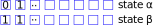
\includegraphics [width=0.7\textwidth] {./imag/exact_corr_of_c_east_model.pdf}
		\setlength{\abovecaptionskip}{0pt}
		\caption{Exact $C(t)$ (solid lines) from \textbf{numerical results} for finite chains (\textbf{Eisinger and Jaeckle, 1991)}.}
	\end{figure}
\end{frame}

\begin{frame}
	\frametitle{{\textcolor{blue}{$\beta$-dependence}} of $C(t)$ (semi-log plot)}
	\begin{figure}
		\centering
		\includegraphics [width=0.9\textwidth] {./imag/beta_dependence_of_corr_N32_step10000.pdf}
		\setlength{\abovecaptionskip}{0pt}
		\caption{{\textcolor{blue}{$t$-dependence}} and {\textcolor{blue}{$\beta$-dependence}} of $C(t)$}
	\end{figure}
\end{frame}
\begin{frame}
	\frametitle{{\textcolor{blue}{$\beta$-dependence}} of $C(t)$ (semi-log plot)}
	\begin{figure}
		\centering
		\includegraphics [width=0.9\textwidth] {./imag/beta_dependence_of_corr_N64_step10000.pdf}
		\setlength{\abovecaptionskip}{0pt}
		\caption{{\textcolor{blue}{$t$-dependence}} and {\textcolor{blue}{$\beta$-dependence}} of $C(t)$}
	\end{figure}
\end{frame}
\begin{frame}
	\frametitle{{\textcolor{blue}{$\beta$-dependence}} of $C(t)$ (semi-log plot)}
 \begin{figure}
	\centering
	\includegraphics [width=0.6\textwidth] {./imag/beta_dependence_of_corr_N128_step10000_p2p4.pdf}
	\setlength{\abovecaptionskip}{0pt}
	\caption{$C(t)$ for $c=0.2$({\textcolor{green}{green}}) and $c=0.4$({\textcolor{blue}{blue}}) in our simulations  are agree with the simulation results in \textbf{Pitts, Young and Andersen,2000}.}
\end{figure}
$\rightarrow$ For $c < 0.5$, our MC simulations are correct! 

Question: Why we can not generate $c >0.5$ in the MC simulations?
\end{frame}

\begin{frame}
	\frametitle{{\textcolor{blue}{$\beta$-dependence}} of $C(t)$ (semi-log plot): Test 1}
	\textbf{J-E (EMA) theory provides an excellent fit to the data at higher} $c$ and \textbf{fits short time data well at lower} $c$'s, but ultimately fails because the EMA correlator dost not decay to 0 for $c<0.5$
	
	Kawasaki (MCA) theory is less accurate at all $c$'s, predicting relaxation that is \textbf{too rapid at short times} at all $c$'s and then predicting \textbf{a failure to relax to 0 at long times for low $c$'s}. (\textbf{Pitts, Young, and Andersen,2000} )     
	\begin{figure}
		\centering
		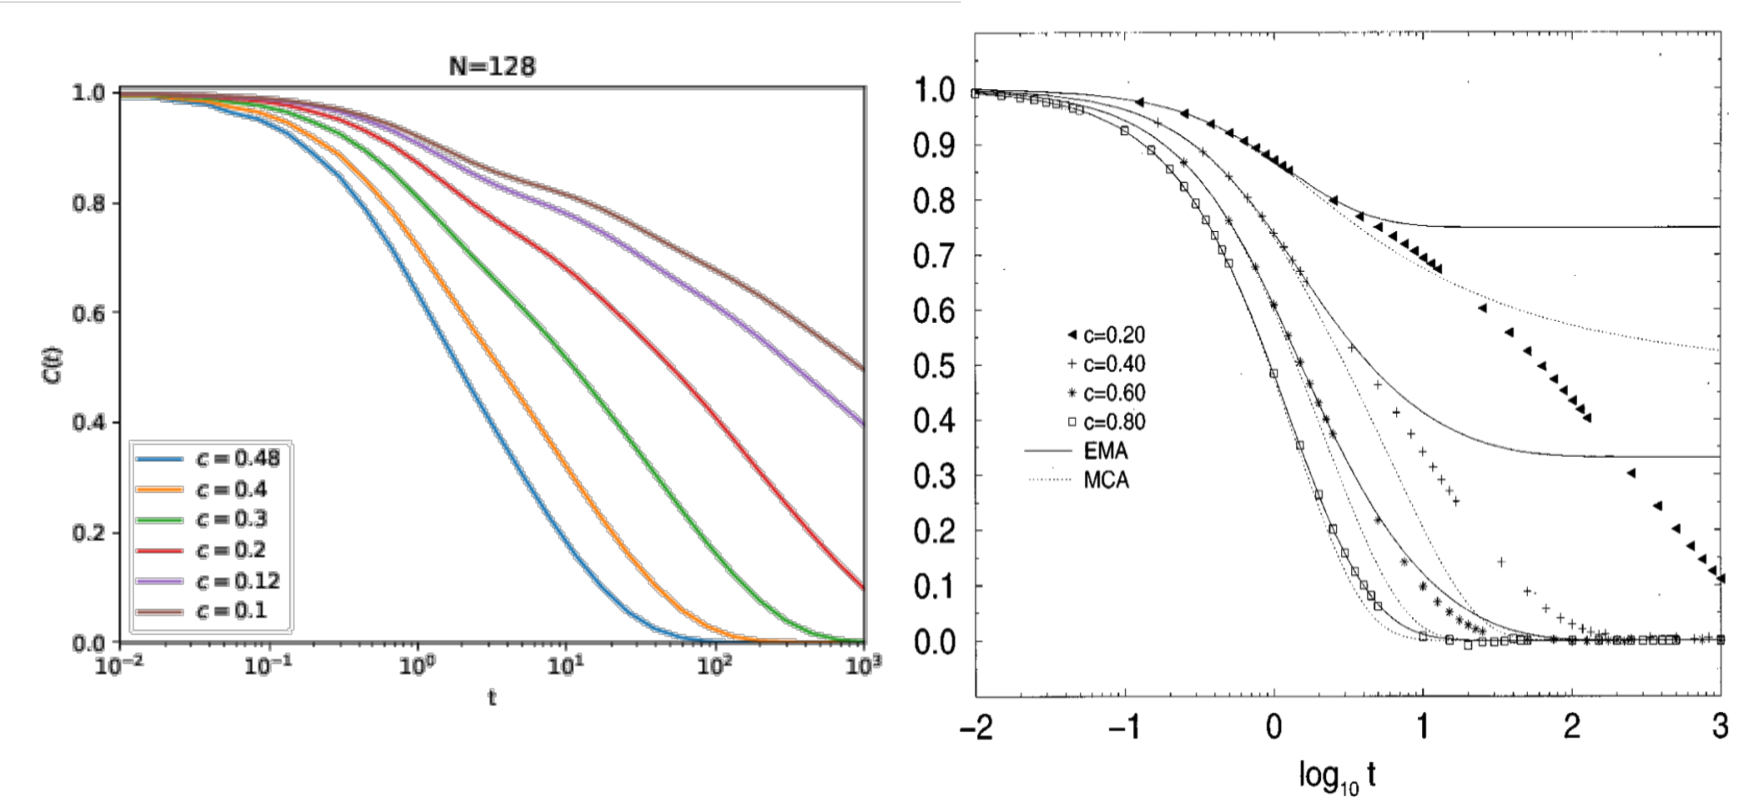
\includegraphics [width=0.9\textwidth] {./imag/beta_dependence_of_corr_N128_step10000_b.pdf}
		\setlength{\abovecaptionskip}{0pt}
		\caption{ (Left) $C(t)$ for different $c$'s in our simulations and (Right) the simulation results in \textbf{Pitts, Young and Andersen,2000}, \textbf{EJ} (solid), and \textbf{Kawasaki} (dotted). }
	\end{figure}
\end{frame}

\begin{frame}
	\frametitle{{\textcolor{blue}{$\beta$-dependence}} of relaxation time $\tau$}
	\begin{figure}
		\centering
		\includegraphics [width=0.7\textwidth] {./imag/relaxation_time_of_corr_on_beta_N128_step10000.pdf}
		\setlength{\abovecaptionskip}{0pt}
		\caption{{\textcolor{blue}{$\beta$-dependence}} of $C(t)$. $N=128$.}
	\end{figure}
\end{frame}

\begin{frame}
	\frametitle{{\textcolor{blue}{$c$-dependence}} of relaxation time $\tau$}
	\begin{figure}
		\centering
		\includegraphics [width=0.7\textwidth]
		{./imag/relaxation_time_of_corr_on_c_N128_step10000.pdf}
		\setlength{\abovecaptionskip}{0pt}
		\caption{{\textcolor{blue}{$c$-dependence}} of $C(t)$. $N=128$.}
	\end{figure}
\end{frame}

%\section{Size effects}
%\begin{frame}
%	\frametitle{{\textcolor{blue}{$c$-dependence}} of $C(t)$.}
%	\begin{figure}
%		\centering
%		\includegraphics [width=0.7\textwidth]
%		{./imag/N_dependence_of_corr_beta2.00_step2400.pdf}
%		\setlength{\abovecaptionskip}{0pt}
%		\caption{{\textcolor{blue}{$N$-dependence}} of $C(t)$ is not obvious in these simulations.}
%	\end{figure}
%\end{frame}

\section{Conclusions}
\begin{frame}
	\frametitle{For $C(t)$: Test the program}
    %\begin{itemize}  
    %	\item 
    %	%\item $\tau(\beta) \sim  \exp(\beta^2 \ln2)$ (\textbf{Sollich, Evans PRE 2003})
    %\end{itemize}	
    	\begin{figure}
    	\centering
    	\includegraphics [width=0.7\textwidth]
    	{../../N_beta_mp_blocking/imag/beta_dependence_of_corr_N9_step10000_log_blocking_and_pbc.pdf}
    	\setlength{\abovecaptionskip}{0pt}
    	\caption{ The relaxation of $C(t)$ for 1D East chain with blocking boundary ($N=9$) is slower than that with PBC. While, $C(500)=0.06$ in \textbf{Jaeckle1991}. We get different values $C(500) = 0.25$, Why? (Here we use $N=9$ for this blocking boundary. The result also different from that in  \textbf{Jaeckle1991}.)}
    \end{figure}
\end{frame}

\section{Appendix}
\begin{frame}
	\frametitle{Concepts: Definition of the East model}
	\begin{itemize}
		\item There are no static interactions between spins, but there is an energy difference between the spin up and spin down states for each spin: $\Delta E= E_{1}- E_{-1}$.
		\item The energy difference $\Delta E/T$ determines $c$ ($c$ is the equilibrium concentration of up spins at any temperature). $\Delta E$ is a constant in the East model, so the energy difference can be written as $1/T$, or $\beta$. 
		\item $\beta$ is the ratio of energy difference $\Delta E=1$ and $k_\text{B}T=T$.
		\item The thermodynamic state is specified by a single state variable $c$.
		\item $c$ is also the probability that any particular spin is up.  
		
	\end{itemize}	
\end{frame}
\begin{frame}
	\frametitle{Concepts: Facilitating set}
	\begin{itemize}
		\item In each model, for each site $i$ there is a set of $f$ neighboring sites $S(i)$ s.t. the spin on site $i$ can flip only if all the spins on the sites $S(i)$ are up.
		\item \textbf{Facilitating set} $S(i)$ of site $i$ for the East model: spin $i+1$.
		
	\end{itemize}	
\end{frame}

\begin{frame}
	\frametitle{A simplifying case}
	Definitions:
	\begin{itemize}
		\item The \textbf{state} $\Gamma$ of a system of $N$ spins is specified by $n_1 ,\cdots,n_N$;
		\item The possible transitions of the system are those in which
		a single spin flips; 
		\item The flip rate for spin $i$ depends on the state of  spin $i+1$.
	\end{itemize}	
	Assumptions:
	\begin{itemize}
		\item The spins are statistically independent at equilibrium;
		%\item  All \textbf{sites} have the \textbf{same distribution function} for the occupation number, ie, $\forall i,  t=\infty,  p(n_i=0)= 1-e^{-\beta}, p(n_i =1) = e^{-\beta}$?
		\item  All \textbf{sites} have the \textbf{same distribution function} for the occupation number, ie, $\forall i,  t=\infty,  p(n_i=0)= 1-c, p(n_i =1) = c$;
		\item $\rho_0(\Gamma) = \prod_{i=1}^N p(n_i)$.
	\end{itemize}	
\end{frame}

\begin{frame}
	\frametitle{For $C(t)$:}
	\begin{itemize}
		\item $\phi(t) = \frac{\langle \delta n_i(t) \delta n_i(0)\rangle}{c(1-c)}$ (\textbf{Eisinger and Jaeckle, 1991}, where $\sigma_i =\pm 1$).
		\item   $C(t) = \frac{\langle\delta n_i(t)\delta n_i (0)\rangle}{\langle \delta n_i(0)^2 \rangle}$. What is the difference between $C(t)$ and $\phi(t)$ ?  
		
	    $C(t)=\phi(t)$. ($n_i = 0 \text{ or } 1$)
		\item $C(t)$ can also be written as $\frac{P(s_i(t=1)| s_i(t=1))-c}{1-c}$.
		
		\item $c=\langle n_i \rangle =0.9, 0.8$ (CHECK THIS PROBLEM! ?)
		\item At low $T$, $c$ is small (\textbf{Sollich 2003}).
		\item For $N\to \infty$, all boundary conditions (free BC, blocking BC (\textbf{JCP, 113,8671}) and PBC) gives the \textbf{same} result of $C(t)$! (\textbf{Pitts, Young, Andersen, 2000, JCP, 113,8671})  
	\end{itemize}	
\end{frame}

\begin{frame}
	\frametitle{The up-spin persistence function $P_1(t)$}
	\begin{itemize}
		\item In $[0,t]$, $s_{i-1}$ has been up a fraction $m$ of the time, and the evolution of $s_i$ has been that (evolution) of a single spin over time $mt$.
		\item $P(m,t)$: The distribution of $m$ for a given $t$ by $P(m;t)$. What's does $P(m,t)$ mean? A: There are two possible answers. \textbf{(1)} Perform one MC simulation, spin $s_{i-1}$, $i =0,\cdots, N-1$,  has been up $m_i$ times. The distribution of $m_i$ is $P_\text{space}(m; t)$; \textbf{(2)} Perform $X$ times simulations, for site $i$, the spin $s_{i-1}$ have $m_x$ times up state. The distribution of $m_x$ is $P_\text{time}(m;t)$.     
         (\textbf{Sollich 2003}).
         \item \textbf{Question}: Is the $P_\text{time}(m;t)$ identical to $P_\text{space}(m;t)$?  Answer and prove. 
	\end{itemize}	
\end{frame}

\begin{frame}
	\frametitle{Theoretical object: to derive an equation of $C(t)$ (kinetic theory of $C(t)$)}
	In general,
	\begin{alignat}{3}
		\frac{dC(t)}{dt} + \omega C(t) + \omega^{-1} \int_0^t d\tau M^\text{irr}(t-\tau) \frac{dC(\tau)}{d\tau} = 0,
	\end{alignat}
where $\omega = k(0)$, $k(t) = -\frac{dC(t)}{dt}$, $M^\text{irr}$ is irreducible memory function.  (\textbf{Pitts, Andersen 2000})

In MCT, assume that
\begin{alignat}{3}
M^\text{irr}(t)=\sum_n a_n(c) [C(t)]^n. 
\end{alignat}
Some approximations:
\begin{itemize}
	\item  $M^\text{irr}_\text{K}(t) = c(1-c) [C(t)]^2$ (\textbf{Kawasaki1995})
	\item  $M^\text{irr}_\text{EJ}(t) = c(1-c) C(t) $ (\textbf{Eisinger and Jaeckle 1993} )
	\item diagrammatic representations of the irreducible memory function $\to$ obtained the irreducible memory kernel from a set of irreducible diagrams: $M^\text{irr} = c(1-c) C(t)$ for $(c< 0.5)$ (\textbf{Pitts, Young, Andersen, J. Chem. Phys. 2000, 113, 8671})
	 (\textbf{Pitts and Andersen, 2001})
	 \item A matrix formalism defined in the complete dynamic phase space (\textbf{Wu, Cao, J. Phys. Chem. B 2004, 108, 6796}).% (inspired by Pitts and Andersen).
\end{itemize}	
\end{frame}

\begin{frame}
	\frametitle{More about  $C(t)$: Detailed balance}
	Let the state $\alpha = (s_1,s_2,\cdots,s_N)$. In equilibrium,
	
	$ \frac{\partial P_\alpha(t)}{\partial t} = 0 \Rightarrow$ $P_\alpha(t) W_{\alpha\to \beta} = P_\beta(t) W_{\beta\to \alpha}$, where
	\begin{itemize}
		\item $P_\alpha(t)$ is the probability of the chain being in state $\alpha$.
		\item From detailed balance,$W_{a\to b} = e^{-\beta}$; $W_{b\to a} = 1 \Rightarrow$ 
		
		$P_b(t)/ P_a(t) = e^{-\beta}$ (see Figure).
	\end{itemize}	
	\begin{figure}
	\centering
	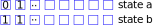
\includegraphics [width=0.4\textwidth]
	{./imag/detailed_balance_east_model.pdf}
	\setlength{\abovecaptionskip}{0pt}
	\caption{Two states of the 1-D finite East model with $N$ sites. }
    \end{figure}

\end{frame}

\begin{frame}
		\frametitle{More about  $C(t)$: Detailed balance condition (In general)}
We now restrict attention to systems for which there is a stationary distribution function
$\rho_0(\Gamma)$ s.t. the transition probabilities obey the DBC (\textbf{Pitts and Andersen, 2001}):
\begin{alignat}{3}
W(\Gamma',\Gamma) \rho_0(\Gamma) =W(\Gamma,\Gamma') \rho_0(\Gamma').
\end{alignat}

\end{frame}
\end{document}
